\documentclass[UTF8,fontset=fandol]{article}
\title{猫站小报 第 1 期}
\author{猫站小报编辑部}
\date{\today}
\usepackage{ctex}
\usepackage{indentfirst}
\setlength{\parindent}{2em}
\usepackage{listing}
\usepackage{xcolor}
\usepackage{graphicx}
\usepackage{geometry}
\geometry{left=0.3in,right=0.3in,top=0.3in,bottom=0.3in}

\begin{document}
\maketitle
\section{编辑部专版}

\pagebreak

\section{积木纪元}
\subsection{作品A}
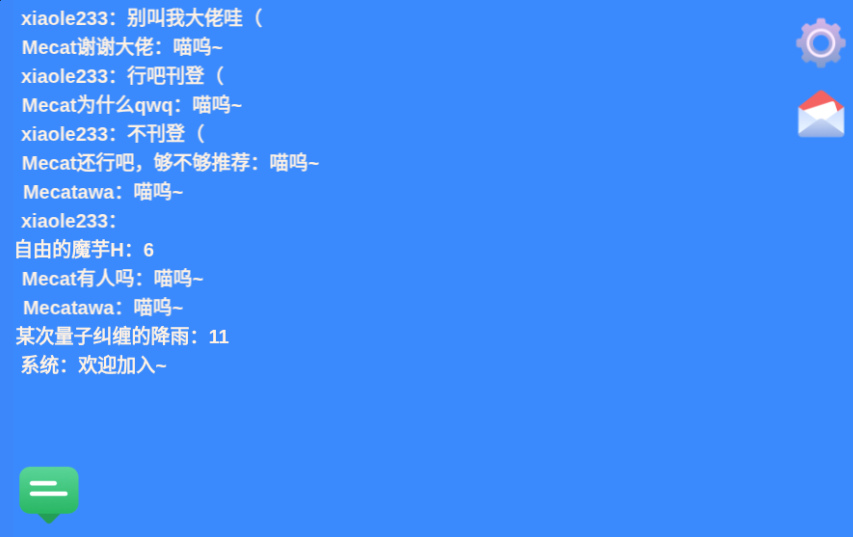
\includegraphics[width=0.5\textwidth]{assets/01/kitten-1.png}

\noindent
\textbf{作者:} \\
\textbf{ID:} \\
\textbf{介绍:} \\
\textbf{编辑评:}
\hfill
\includegraphics[width=0.08\columnwidth]{assets/01/kitten-1-qrc.png}
\subsection{作品B}
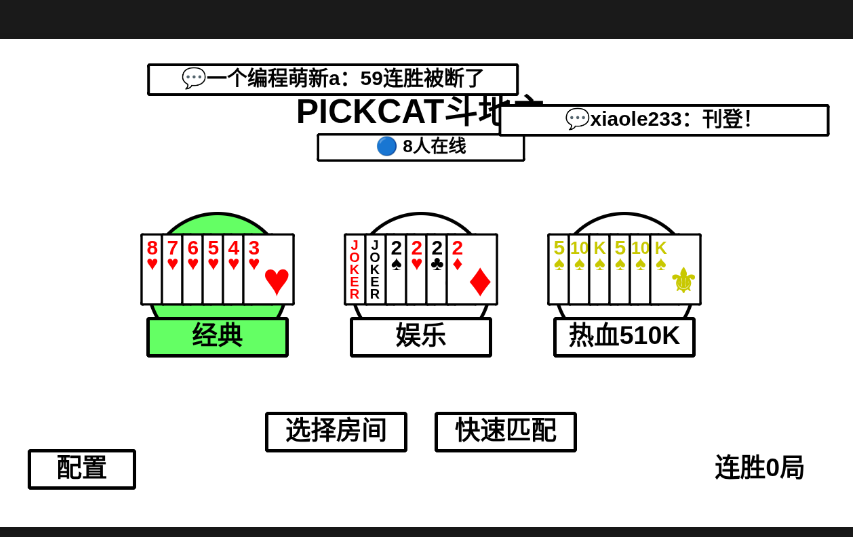
\includegraphics[width=0.5\textwidth]{assets/01/kitten-2.png}

\noindent
\textbf{作者:} \\
\textbf{ID:} \\
\textbf{介绍:}\\
\textbf{编辑评:}
\hfill
\includegraphics[width=0.08\columnwidth]{assets/01/kitten-2-qrc.png}

\pagebreak
\section{代码诗篇}
\subsection{作品A}
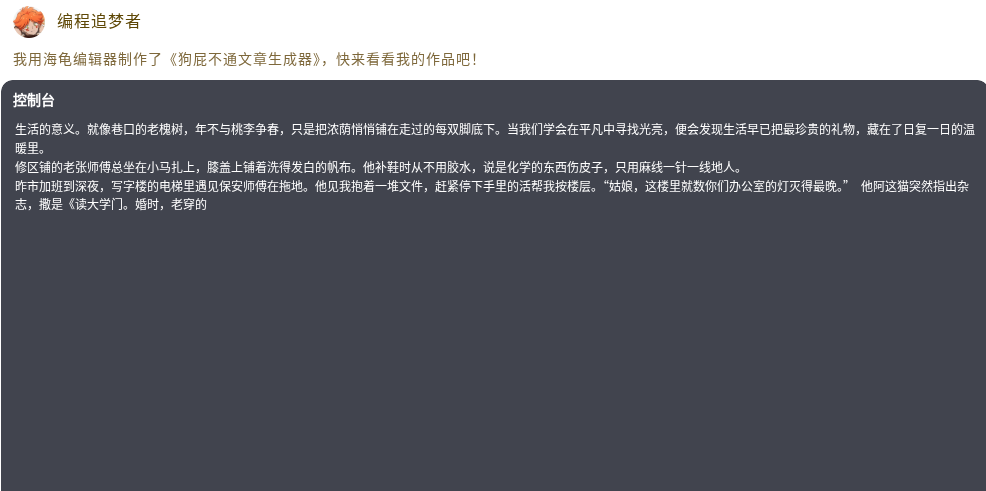
\includegraphics[width=0.5\textwidth]{assets/01/python-1.png}

\noindent
\textbf{作者:} \\
\textbf{作品ID:} \\
\textbf{介绍:}\\
\textbf{编辑评:}
\hfill 
\includegraphics[width=0.08\columnwidth]{assets/01/python-1-qrc.png}

\subsection{作品B}
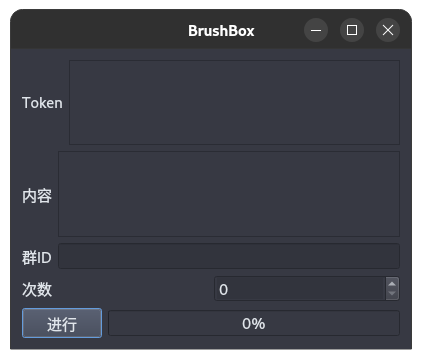
\includegraphics[width=0.5\textwidth]{assets/01/python-2.png}

\noindent
\textbf{作者:} \\
\textbf{Github仓库地址:} \\
\textbf{介绍:}\\
\textbf{编辑评:}
\hfill 
\includegraphics[width=0.08\columnwidth]{assets/01/python-2-qrc.png}

\pagebreak
\section{传火者}
\begin{center}
	\zihao{-1}
	\textbf{标题}
	\normalsize
	供稿:
\end{center}


\section{后记}
\paragraph{编辑} 目前唯一编辑也是主笔:xiaole233 邮箱地址:xiao\_2010@outlook.com
\paragraph{版权说明} 刊登的所有作品及文章均以取得原作者同意。\\ 
猫站小报 第一期  © 2025 by 小报编辑部 is licensed under CC BY 4.0.\\ To view a copy of this license, visit https://creativecommons.org/licenses/by/4.0/

\end{document}